\section{Datenbankmodelle für Entwurf}
\label{sec:entwurf}

\paragraph{Entity-Relationship-Modelle}
\begin{itemize}
	\item \textbf{Entity}: Objekt der Real-/Vorstellungswelt (z.B. Buch)
	\item \textbf{Relationship}: Beziehung zw. Entities (z.B. Schüler hat Buch)
	\item \textbf{Attribut}: Eigenschaft von Entities (z.B. ISBN)
\end{itemize}
\begin{figure}[H]\centering\label{EntityRelationship}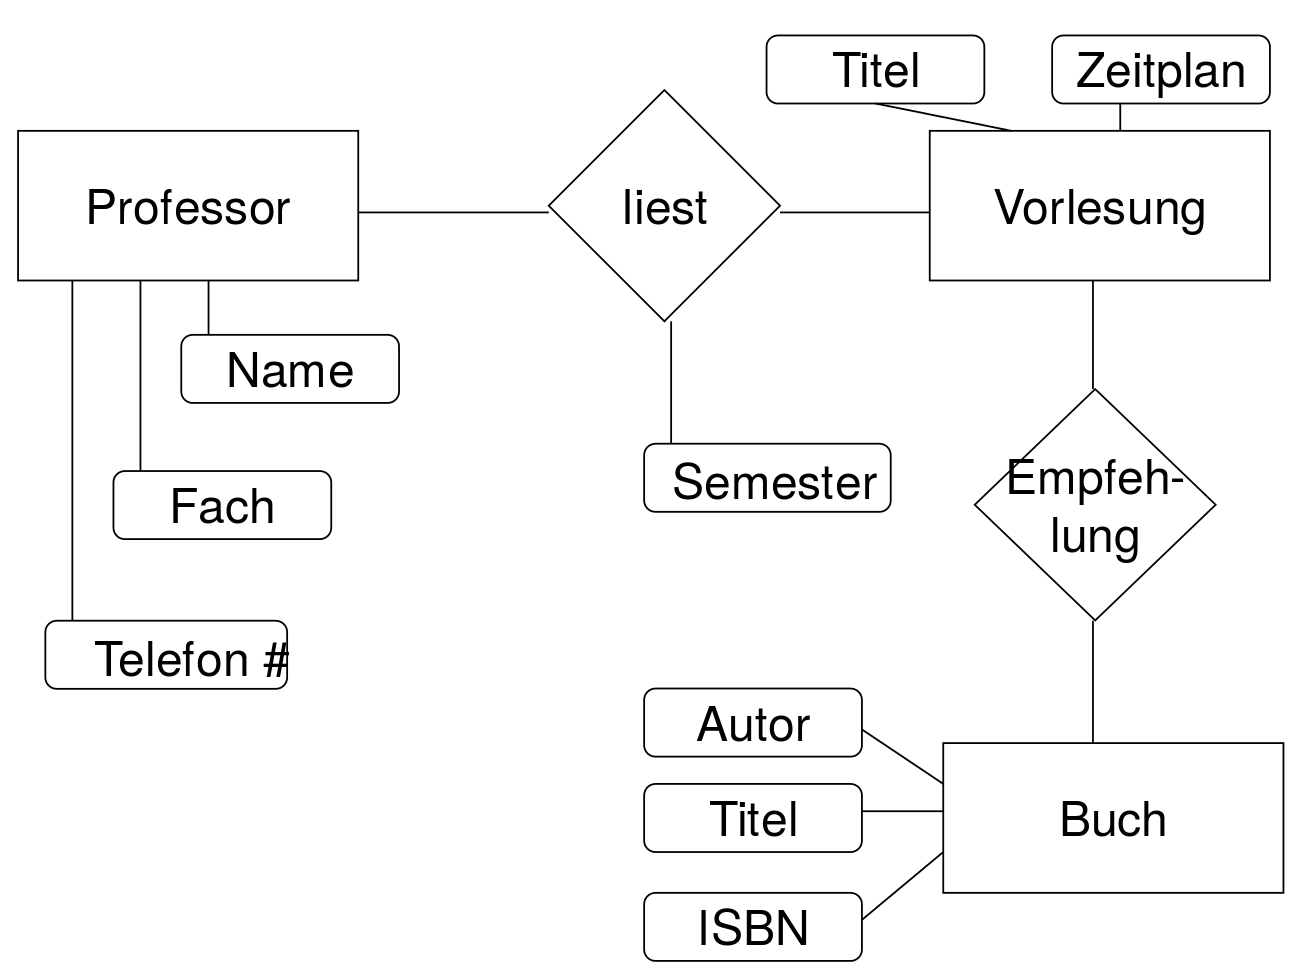
\includegraphics[width=.5\linewidth]{EntityRelationship}\end{figure}

\paragraph{Attribute}
\begin{itemize}
	\item \textbf{Mengenwertig:} Durch Doppelrand gekennzeichnet
	\item \textbf{Optional:} durch Kreis auf Attribut-Verbindung gekennzeichnet
\end{itemize}

\paragraph{ER --- Modellierungskonzepte}
\begin{itemize}
	\item \( \mu(D) \): Interpretation von \( D \), mögliche Werte einer Entity-Eig.
	\item \( \mu \)(\lstinline[language=sql]{int}): \( \mathbb{Z} \),  \( \mu \)(\lstinline[language=sql]{string}): \( C^\star \) (Folgen von Zeichen aus \( C \))
	\item \( \mu(E) \): Menge der möglichen Entities vom Typ \( E \)
	\item \( \sigma_i \)(E): Menge der \emph{aktuellen} Entities vom Typ \( E \) in Zustand \( \sigma\)
	\\* \( \leadsto \) \( \sigma(E) \subseteq \mu(E) \) und \( \sigma(E) \) endlich
	\item \( \mu(R) = \mu(E_1) \times \cdots \times \mu(E_n) \) \\* \( \leadsto \) Die Menge aller möglichen Ehen ist die Menge aller (Mann,Frau)-Paare.
	\item \( \sigma(R) \subseteq \sigma(E_1) \times \cdots \times \sigma(E_n) \) \\* \( \leadsto \) aktuelle Beziehungen nur zwischen aktuellen Entities
	\item Attribut \( A \) eines Entity-Typen \( E \) ist im Zustand \( \sigma \) eine Abbildung \( \sigma(A): \sigma(E) \to \mu(D) \) (\textbf{nicht} \( A: \sigma(E) \to \mu(D) \))
	\item Beziehungsattribute: \( \sigma(A): \sigma(R) \to \mu(D) \) (Beziehung \( R \), Attribut \( A \), möglicher Wertebereich \( \mu(D) \))
\end{itemize}

\paragraph{Mehrstellige Beziehungen}
\begin{itemize}
	\item Umwandlung von mehrstelligen Beziehungen in mehrere einstellige Beziehungen i.A. nicht einfach möglich.
\end{itemize}

\paragraph{Funktionale Beziehungen}
\begin{itemize}
	\item Jedem Professor lässt sich ein Zimmer zuordnen, umgekehrt nicht zwingend
	\item Schreibe: \( R: E_1 \to E_2 \)
\end{itemize}
\begin{figure}[H]\centering\label{FunktionaleBeziehung}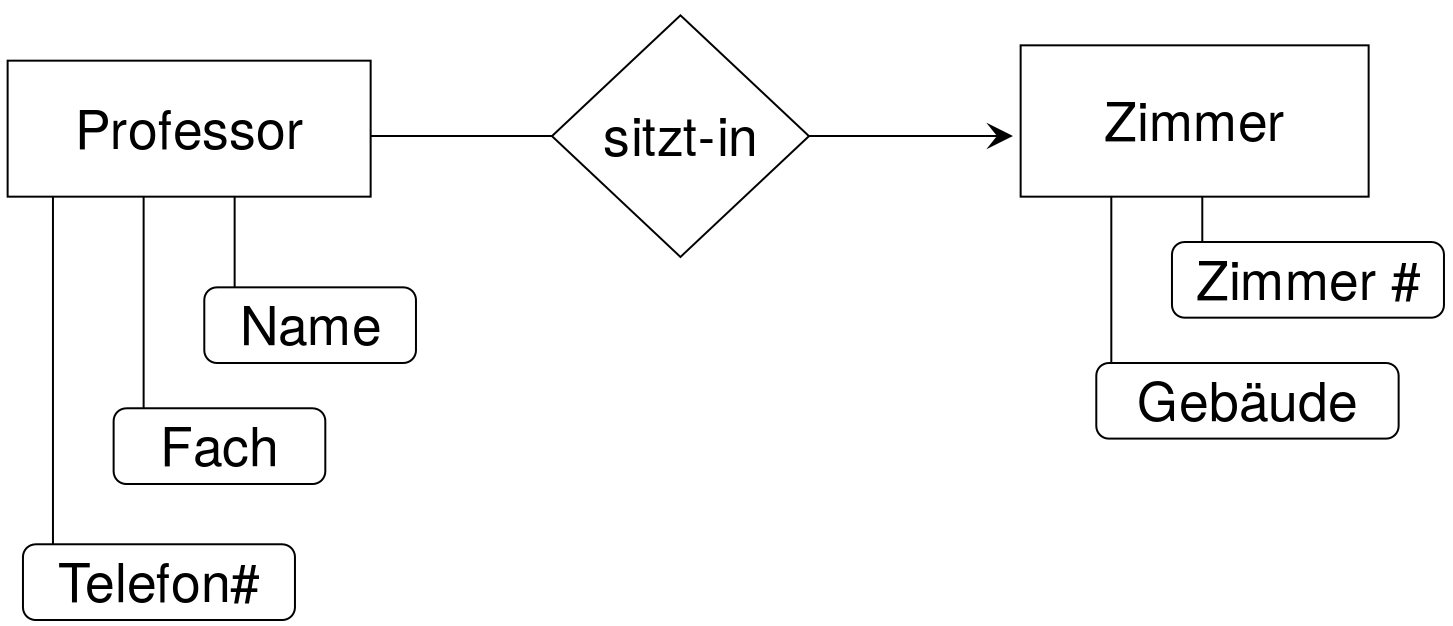
\includegraphics[width=.5\linewidth]{FunktionaleBeziehung}\end{figure}



\paragraph{Schlüssel}
\begin{itemize}
	\item Schlüsselattribute \( \{ S_1, \dots, S_k \} \subseteq \{ A_1, \dots, A_m \} \) für \\* Entity-Typ \( E(A_1, \dots, A_m) \)
	\item Notation: Schlüssel unterstreichen: \( E(\dots, \underline{S_1}, \dots, \underline{S_i}, \dots) \)
	\item Schlüssel ist minimal: Wird ein Schlüsselattribut entfernt, so ist das entstehende Tupel nicht mehr eindeutig
\end{itemize}

\paragraph{Abhängige Entity-Typen}
\begin{itemize}
	\item Identifikation über funktionale Beziehung (als Schlüssel)\\
	Bsp: (Exemplar-)Nummer bezieht sich auf jeweiliges Buch
\end{itemize}
\begin{figure}[H]\centering\label{AbhaengigeEntity}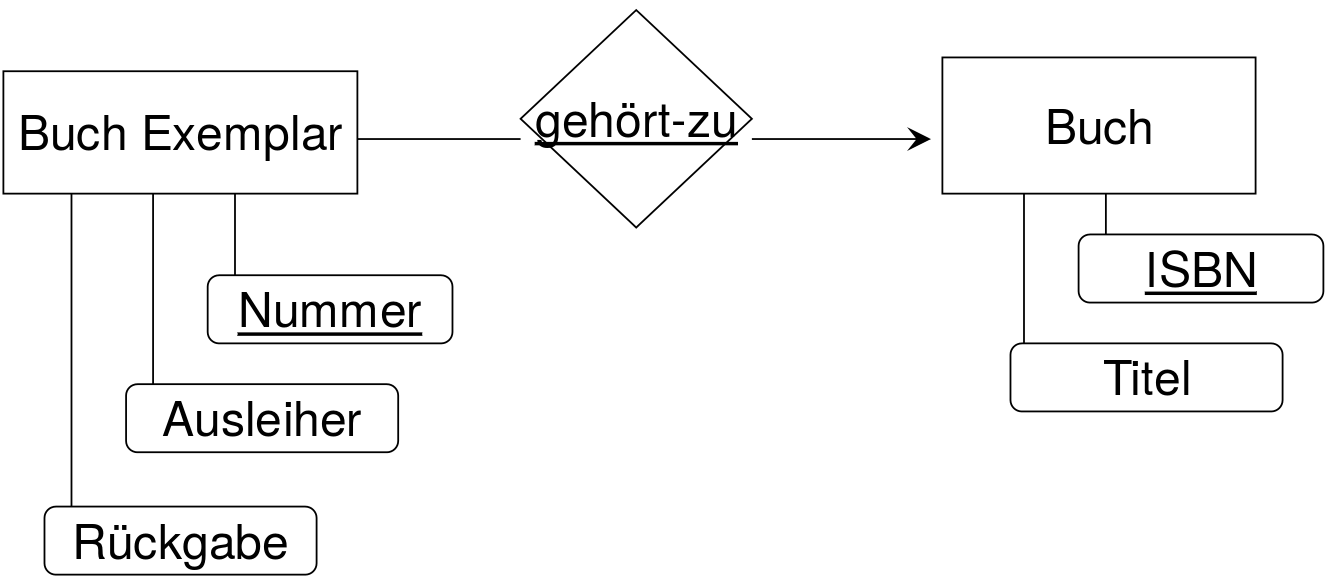
\includegraphics[width=.5\linewidth]{AbhaengigeEntity}\end{figure}

\paragraph{IST-Beziehung}
\begin{figure}[H]\centering\label{ISTBeziehung}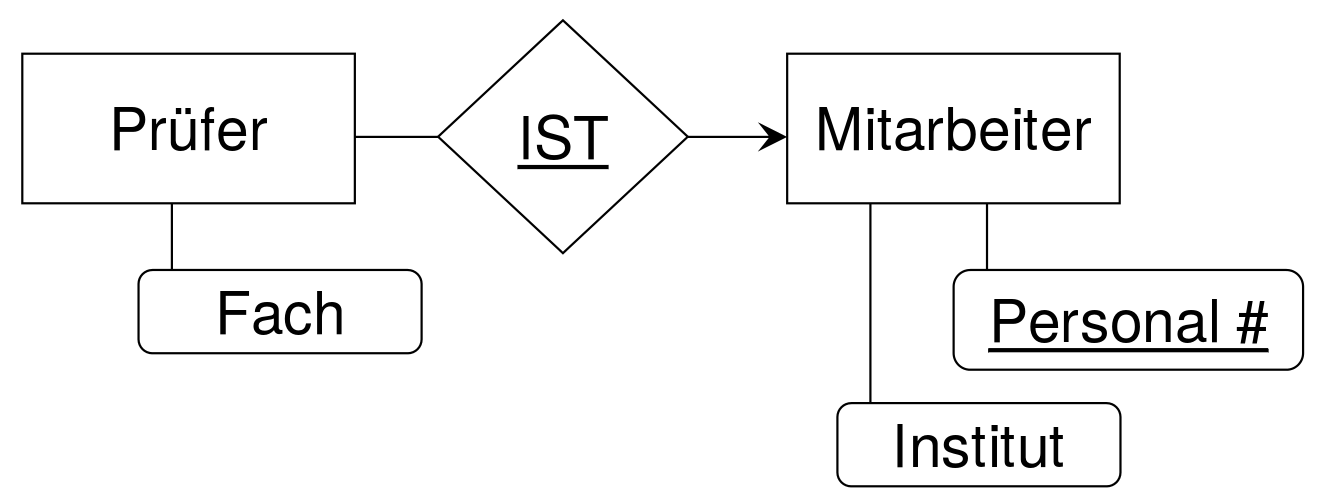
\includegraphics[width=.5\linewidth]{ISTBeziehung}\end{figure}
\begin{itemize}
	\item Spezialfall eines abhängigen Entity-Typen (nur Beziehung als Schlüssel)
	\item Vererbung von Attributen (und Werten): \\* \( \sigma(\text{Prüfer}) \subseteq \sigma(\text{Mitarbeiter}) \)
\end{itemize}
\begin{figure}[H]\centering\label{MehrereFaecher}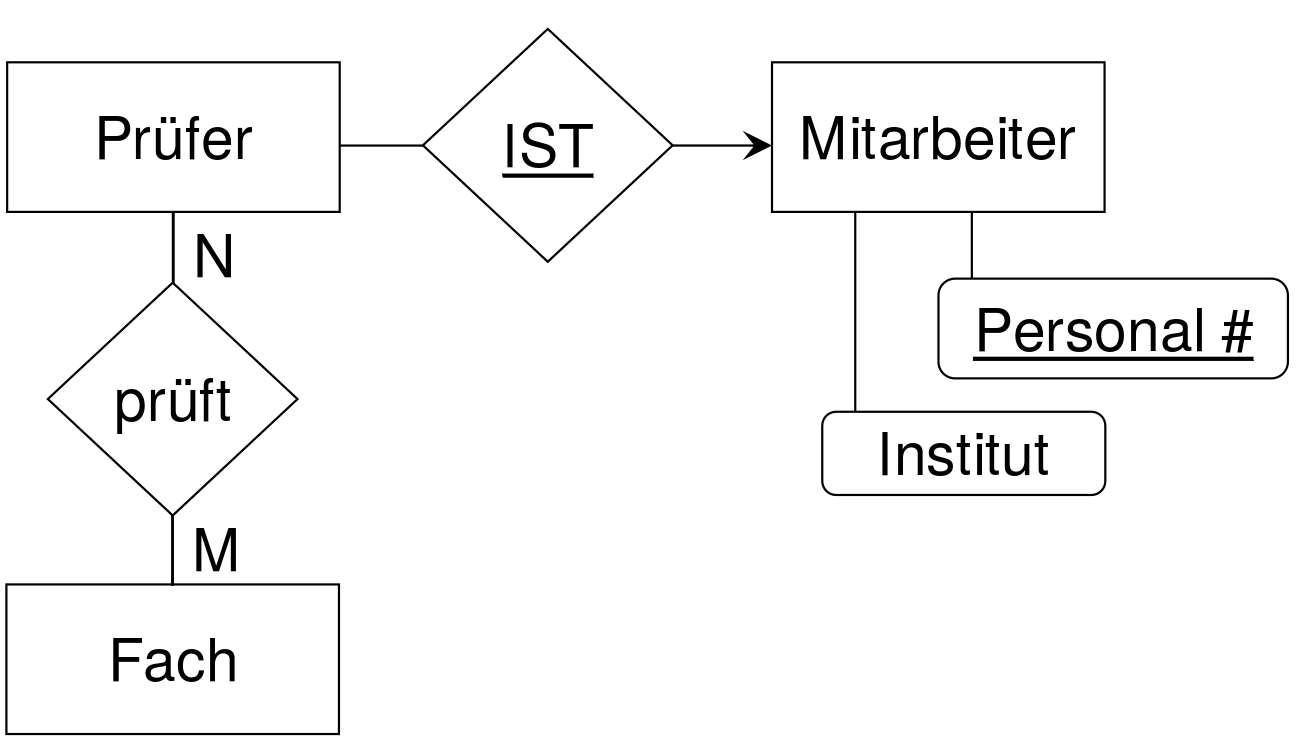
\includegraphics[width=.5\linewidth]{MehrereFaecher}\end{figure}

\paragraph{Entwurf --- Kardinalitäten}
\begin{itemize}
	\item An wv. Beziehungen muss Entity teilnehmen? \( \leadsto \) einschränken
	\item \textbf{Teilnehmerkardinalität}: \lstinline[language=sql]{arbeitet_in(Mitarbeiter[0,1],Raum[0,3])} \\*
		- jeder Mitarbeiter hat einen oder keinen zugeordneten Raum \\*
	 	- pro Zimmer arbeiten maximal drei Mitarbeiter \\*
	 	- ein Zimmer kann leerstehen
	 \item \textbf{Standardkardinalität}: 1 Mannschaft steht mit 11 Spielern in Bezug \\*
	 Auch hier Intervallangabe möglich\\*
	  Speziell: \lstinline[language=sql]{m:n}/\lstinline[language=sql]{1:n}/\lstinline[language=sql]{1:1}-Beziehung (Untere Schranke jeweils \emph{0})
	 \begin{figure}[H]\centering\label{Mannschaft}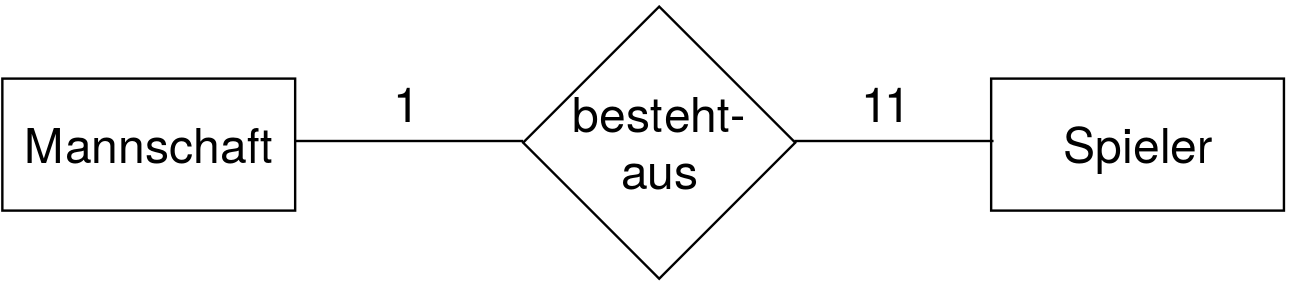
\includegraphics[width=.5\linewidth]{Mannschaft}\end{figure}
\end{itemize}





\paragraph{Semantische Beziehungen}
\begin{itemize}
	\item \textbf{Spezialisierung}: \lstinline[language=sql]{Pruefer} Spezialisierung von \lstinline[language=sql]{Mitarbeiter} \\* \( \leadsto \) Vererbung (IST-Beziehung)
	\item \textbf{Partitionierung}: Spezialfall der Spezialisierung, mehrere \emph{disjunkte} Entity-Typen (z.B. Partitionierung von Buch in Monographie und Sammelband)
	\item \textbf{Generalisierung}: Buch oder DVD als Medium \\*
	\lstinline[language=sql]{Medium} ist stets \lstinline[language=sql]{DVD} oder \lstinline[language=sql]{Buch} \\* Aber: Buch muss kein Medium sein.
	\item \textbf{Aggregierung}: \lstinline[language=sql]{Auto} besteht aus \lstinline[language=sql]{Motor}, \lstinline[language=sql]{Karosserie},... \\* \( \leadsto \) Entity aus Instanzen anderer Entity-Typen zusammengesetzt
	\item \textbf{Sammlung} (auch Assoziation): \lstinline[language=sql]{Team} ist Gruppe von \lstinline[language=sql]{Person} \\* \( \leadsto \) Mengenbildung
\end{itemize}

\paragraph{EER}
\begin{itemize}
	\item = Erweitertes ER-Modell
	\item Übernommen: Werte, Entities, Beziehungen, Attribute, Funktionale Beziehungen, Schlüssel (jetzt ausgefüllter Kreis)
	\item Nicht übernommen: IST-Beziehung --- ersetzt durch \emph{Typkonstruktor}
\end{itemize}

\paragraph{EER --- Typkonstruktor}
\begin{itemize}
	\item Ermöglicht Spezialisierung, Generalisierung, Partitionierung
	\item Eingabetypen mit Dreiecksbasis verbunden (bei Generalisierung spezielle Typen, bei Spezialisierung/Partitionierung allgemeine Typen)
	\item Ausgabetypen mit Spitze verbunden
\end{itemize}
\begin{center}
	\begin{figure}[H]\centering\label{SpezialisierungEER}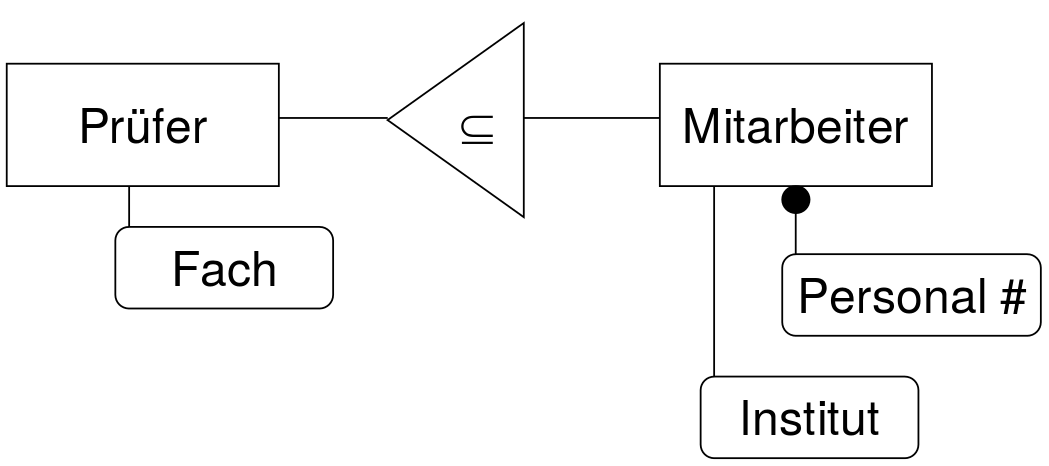
\includegraphics[width=.5\linewidth]{SpezialisierungEER}\end{figure}
	Spezialisierung
	\begin{figure}[H]\centering\label{GeneralisierungEER}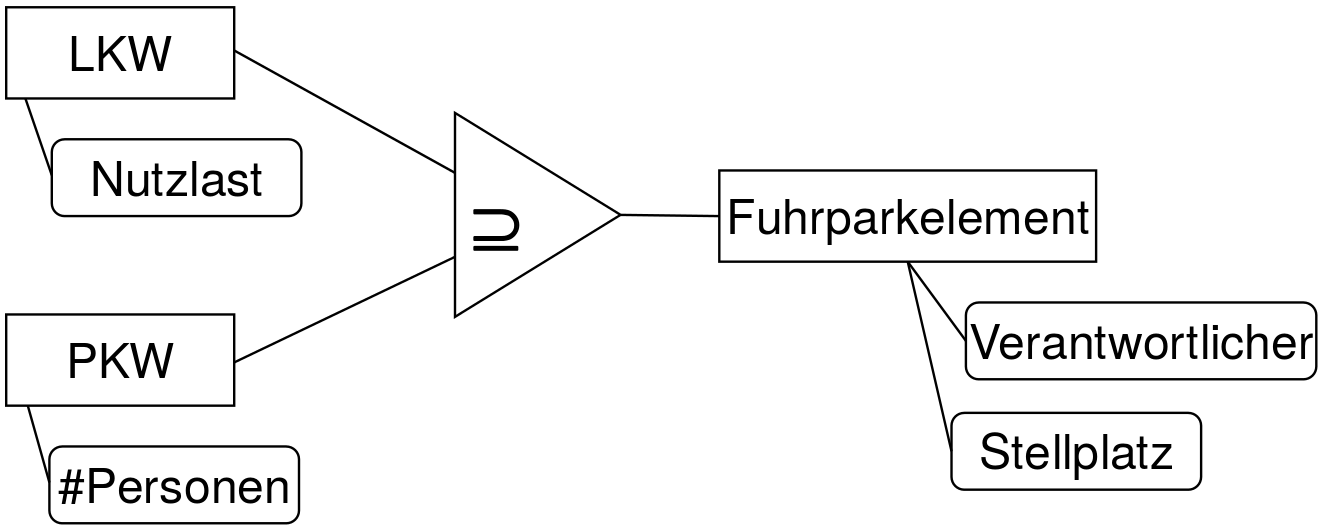
\includegraphics[width=.5\linewidth]{GeneralisierungEER}\end{figure}
	Generalisierung
	\begin{figure}[H]\centering\label{MehrfacheSpezialisierungEER}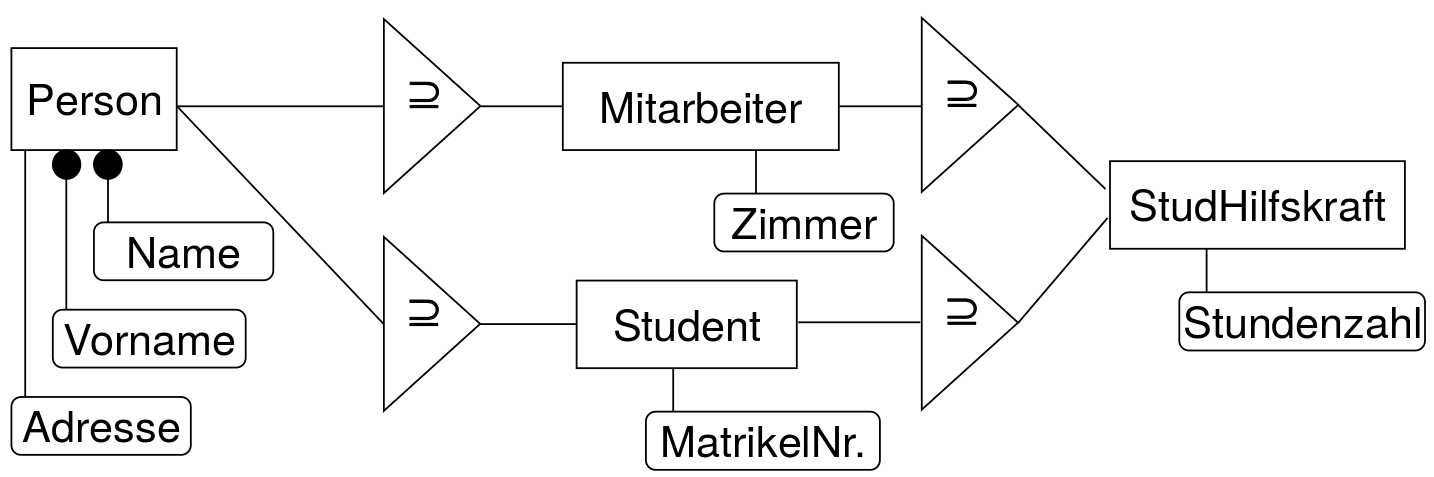
\includegraphics[width=.5\linewidth]{MehrfacheSpezialisierungEER}\end{figure}
	Mehrfache Spezialisierung
\end{center}

\begin{fragen}
	\item Wie ist die Semantik von Datenmodellen definiert?
	\item Geben Sie ein Beispiel für mehrstellige Beziehungen an und erläutern Sie, warum der Sachverhalt mit mehreren zweistelligen Beziehungen nicht korrekt darstellbar wäre.
	\item Welche semantischen Beziehungen aus dem EER-Kontext kennen Sie? Erläutern Sie die Unterschiede und geben Sie jeweils ein Beispiel an.
\end{fragen}
